%************************************************
\chapter{The LUX Detector}

\label{ch:LUX} % $\mathbb{ZNR}$
%************************************************

\section{Detector Components}
\subsection{Cryostat}
\subsection{PMTs}
\subsection{Water Tank}
\subsection{Trigger and Data Acquisition}

\section{Calibrations}
\subsection{Energy}
Two or more calibration line sources of different energies are used to fit for $g_{1}$ and $g_{2}$. The \ac{LUX} experiment uses a suite of sources to calibrate the detector, the sources used to calibrate the energy response of the detector for Run03 are shown in \ref{fig:calib_sources} along with pictoral explanation of the effect of recombination on energy reconstruction.


\begin{figure}[htbp]
\begin{center}
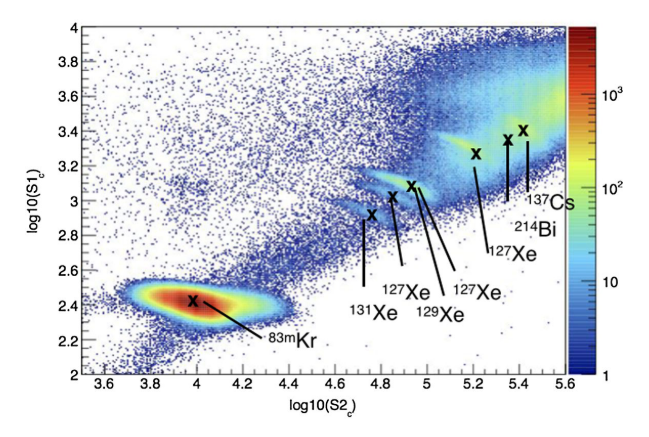
\includegraphics[width=\halffig]{figures/lux/calibration_sources.png}
\caption{Plot showing calibration sources (Figure from \cite{LUX:Run03Comprehensive}. The axis label subscript $c$ denotes corrected variables with calibration for geometrical effects and electron lifetime (this calibration is discussed in further detail in \textbf{ Kr CALIBRATION Section} }
\label{fig:calib_sources}
\end{center}
\end{figure}

The average S1 and S2 of each calibration source is normalized to the true energy:

\begin{equation}
(S1, S2) \longrightarrow \Big(\frac{\langle S1 \rangle}{E}, \frac{\langle S2 \rangle}{E}\Big)
\end{equation}

and a line $y = mx + b$ is fit to the transformed variables, where the slope is $m = -g_{1} / g_{2}$ and the y-intercept is $b = g_{1} / W$. 


\begin{figure}[htbp]
\begin{center}
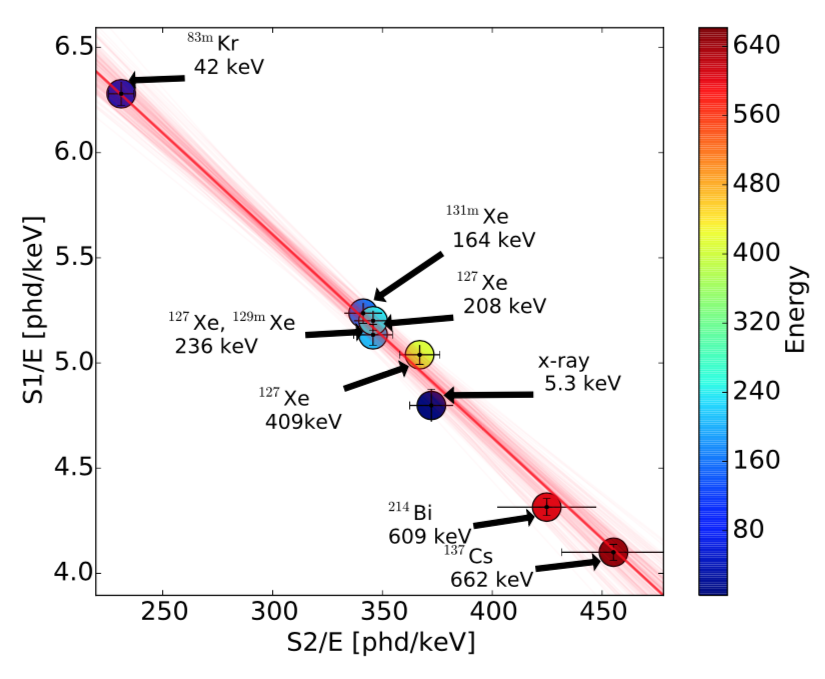
\includegraphics[width=\halffig]{figures/lux/doke.png}
\caption{ Doke plot used to fit $g_{1}$ and $g_{2}$ for LUX Run03 (Figure from \cite{LUX:Run03Comprehensive}}
\label{fig:doke}
\end{center}
\end{figure}


From the fit in Figure~\ref{fig:doke}, the the \ac{LUX} gains were measured to be $g_{1} = 0.117 \pm 0.003$~phd/photon and $g_{2} = 12.1 \pm 0.8$~phd/electron, with an \ac{EEE} of $49\% \pm 3\%$ \cite{LUX:Run03Comprehensive}.

\subsection{Tritium}
\subsection{DD}
\subsection{Kr}




%*****************************************
%*****************************************
%*****************************************
%*****************************************
%*****************************************
